\documentclass{article}
\usepackage[nolist]{acronym}
\usepackage{mathtools}
\usepackage{graphicx}
\usepackage{listings}
\usepackage{pdfpages}


\graphicspath{ {figures/} }

% probably a good idea for the nomenclature entries:
%\acsetup{first-style=bracket}




\title{Analysis of the Effects of non-pointlike Detectors in Hanbury-Brown and Twiss Interferometery }
\author{
        Annina Spescha and David Schenkel \\
        \small Project Report for PHY 243: Computational Astrophysics \\
		\small Supervisor: Prasenjit Saha \\
		\small Department of Physics, University of Zurich\\
}
\date{\today}


\begin{document}
	
\maketitle
% class `abbrev': abbreviations:
\begin{acronym}
  \acro{HBT}{Hanbury Brown and Twiss}
\end{acronym}
\begin{abstract}
In this paper we analyse the effect of spatially extended, non-pointlike, detectors on the measurements of \ac{HBT} Interferometers by simulating measurements done with a disk-shaped detector. We find that the results do not fundamentally change compared to measurements done with point-size detectors, but the contrast gets worse.
\end{abstract}

\section{Introduction}
The \acf{HBT} effect describes the fact that light from an incoherent source when measured at two points will produce a coincidence rate which is slightly higher than the expected Poisson coincidence rate. This additional term in the coincidence rate is the \ac{HBT} effect and it can be used to do intensity interferometry on stars with two detectors as done by Hanbury Brown \& Twiss in 1958 \cite{hbt1958}. More recently, research has been done on the feasibility of using three detectors to recover the phase information a well. Most of this research has been done assuming that only the source has a spatial extent, with the detectors being point-sized. In this paper we analyze if and how detectors with spatial extent affect the result. First we present an analytical solution in a simplified 1-Dimensional double-slit situation with two detectors. We then expand our model into two dimensions where the two point sources are represented by one disk made up of many  point sources and analyze the results for two detectors.

%%%%%%%%%%%%%%%%%%%%%%%%%%%%%%%%%%%%%%%%%%%%%%%%%%%%%%%%%%%%%%

\section{Methods: Expanding the detectors}
\subsection{1-Dimensional Case}
\begin{figure}[ht!]
	\centering
	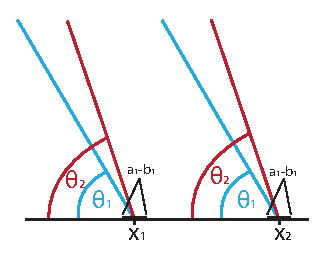
\includegraphics[width=70mm]{figure_2slit}
	\caption{2 detectors (at \(x_1, x_2\)) receiving light from 2 sources with different incident angles \(\theta_1\) and \(\theta_2\) \label{fig:2slit_setup}
	}
\end{figure}
\begin{figure}[ht!]
	\centering
	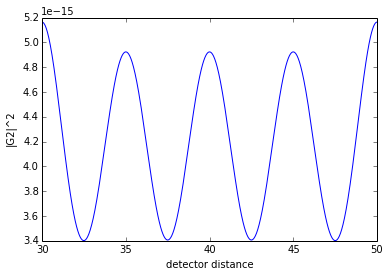
\includegraphics[width=50mm]{1d_detsize_sthan_wave}
	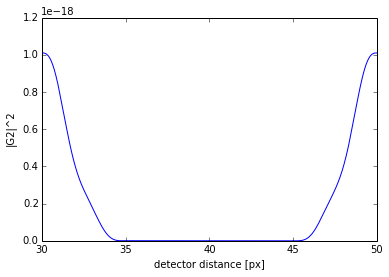
\includegraphics[width=50mm]{1d_detsize_eq_wave}
	\caption{Signal measured at the detector in the case that a) the detector is smaller than the fringe width and b) the detector is about the size of the fringe width and some edge effects\label{fig:1d_detsize}
	}
\end{figure}
In its simplest form, the \ac{HBT} effect can be thought of as Young’s double slit experiment done with an incoherent light source. Roy Glauber \cite{glauber2006} shows that for such a case the correlation at any point on the screen can be expressed by the second order correlation function \[G^{(2)}(x_1 x_2 x_2 x_1) = G^{(1)}(x_1 x_1) G^{(1)}(x_2 x_2) + G^{(1)}(x_1 x_2) G^{(1)}(x_2 x_1)\] where \(G^{(1)}\) are first order correlation functions defined as \[G^{(1)}(x_n x_m) = \langle E^{(-)}(x_n) E^{(+)}(x_m) \rangle\] with \(x_n = r_n t_n\). $x_1$ and $x_2$ are the positions of the two detectors.
\(E^{(\pm)}(x)\) are the two terms to define the oscillating electric field E and can also be expressed as \[E^{(\pm)}(x) = E_{max} e^{\pm i k x }\] 
Since we are only interested in a qualitative analysis, we will omit constant factors such as the amplitude \(E_{max}\) from here on. 

To find \(G^{(2)}\) for 2 detectors with a spatial extent we integrate the individual \(G^{(1)}\) that make up \(G^{(2)}(x_1 x_2 x_2 x_1)\) (See fig. \ref{fig:2slit_setup}) and can then take the absolute value squared to get the signal as measured by detectors with a spatial extent \(b_i-a_i\). The first product, \(G^{(1)}(x_1 x_1) G^{(1)}(x_2 x_2)\), will just yield a constant, hence we can omit this and only integrate
\[\lvert G^{(2)}\rvert^2 =  \lvert{ \int_{a_1}^{b_1} \int_{a_2}^{b_2} G^{(1)}(x_1,x_2) \mathrm{d}x_1 \mathrm{d}x_2 * \int_{a_1}^{b_1} \int_{a_2}^{b_2} G^{(1)}(x_2,x_1) \mathrm{d}x_1 \mathrm{d}x_2 }\rvert^2\]
Where
\[\int_{a_1}^{b_1} \int_{a_2}^{b_2} G^{(1)}(x_1,x_2) \mathrm{d}x_1 \mathrm{d}x_2 \]
\[= \int_{a_1}^{b_1} \int_{a_2}^{b_2} (\mathrm{e}^{ik(x1-x2) \theta_1}\ + \mathrm{e}^{ik(x1-x2) \theta_2}) \mathrm{d}x_1 \mathrm{d}x_2 \]
\[= (\mathrm{e}^{ik(b_1-b_2)\theta_1}-\mathrm{e}^{ik(a_1-b_2)\theta_1}-\mathrm{e}^{ik(b_1-a_2)\theta_1}+\mathrm{e}^{ik(a_1-a_2)\theta_1}) \] 
\[\qquad + (\mathrm{e}^{ik(b_1-b_2)\theta_2}-\mathrm{e}^{ik(a_1-b_2)\theta_2}-\mathrm{e}^{ik(b_1-a_2)\theta_2}+\mathrm{e}^{ik(a_1-a_2)\theta_2})\]
and 
\[\int_{a_1}^{b_1} \int_{a_2}^{b_2} G^{(1)}(x_2,x_1) \mathrm{d}x_1 \mathrm{d}x_2 \]
\[= \int_{a_1}^{b_1} \int_{a_2}^{b_2} (\mathrm{e}^{ik(x2-x1) \theta_1}\ + \mathrm{e}^{ik(x2-x1) \theta_2}) \mathrm{d}x_1 \mathrm{d}x_2\]
\[=(\mathrm{e}^{-ik(b_1-b_2)\theta_1}-\mathrm{e}^{-ik(a_1-b_2)\theta_1}-\mathrm{e}^{-ik(b_1-a_2)\theta_1}+\mathrm{e}^{-ik(a_1-a_2)\theta_1}) \]
\[\qquad + (\mathrm{e}^{-ik(b_1-b_2)\theta_2}-\mathrm{e}^{-ik(a_1-b_2)\theta_2}-\mathrm{e}^{-ik(b_1-a_2)\theta_2}+\mathrm{e}^{-ik(a_1-a_2)\theta_2}) \]

respectively. $x_1$ and $x_2$ are the positions of the two detectors and k is the wave number. $\theta_1$ and $\theta_2$ are the incidence angles (see fig. \ref{fig:2slit_setup}).

To verify our result, we test the case in which the detector size is approximately the same as the fringe width of the interference pattern created by the double slit. As expected, the measured signal drops to zero (See fig. \ref{fig:1d_detsize}).
\begin{figure}[ht!]
	\centering
    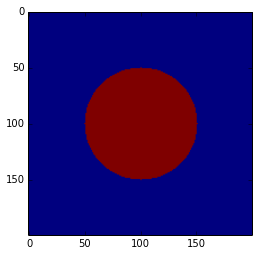
\includegraphics[width=45mm]{figure_source_homo}
    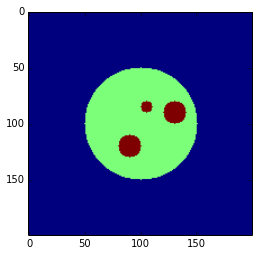
\includegraphics[width=45mm]{figure_source_rand}
    \caption{2-Dimensional disk-shapes used for the analysis: a) homogenous disk used as detectors, b) spotted disk used as source \label{fig:2d_sources}
 }
\end{figure}
The integral is basically a convolution of the expected signal at point detectors convolved with detectors with a spatial extent. Hence, the same result can also be found by taking the inverse fourier transform of \(G^{(1)}(x_1 x_2)\), which then represents the source, and multiplying it with the inverse fourier of the detectors, represented by rect-functions. The multiplication in the position space is equal to the convolution in the fourier space. By taking the fourier transformation and then the absolute value squared of it this yields the same result as our analytical solution, except for a constant factor which has to be added due to the non-steady nature of the (inverse) fast fourier transform functions used to compute the results. In our case this constant factor $\Delta x$ for the fourier transformation and $\Delta x^{-1}$ for the inverse fourier transformation has the order of magnitude of arc seconds respectively arc seconds$^{-1}$. It has to verify the relation $N\Delta x\Delta k=2\pi$ where N is the size of our position space, which corresponds to 512 units of space (pixels) in our case. $\Delta k$ is the correction constant in the fourier space.
\subsection{2-Dimensional Case}
In the 2-Dimensional case the source is not a double slit anymore but a disk made up of individual point sources. This source can either be homogenous or an inhomogenous source with different valued spots (see fig. \ref{fig:2d_sources}, modelled after \cite{wentz2014}). The sources are being created by the function \textit{source2d} and \textit{randsource2d} respectively (See Appendix A).

The detectors are also modelled with a uniform disk. Because they move and detect in k-space they are disks in the fourier space. We then multiply the source with the inverse fourier transformation of the detectors and transform it back in the fourier space to get \(G^{(2)}\) for the 2d case. 


%%%%%%%%%%%%%%%%%%%%%%%%%%%%%%%%%%%%%%%%%%%%%%%%%%%%%%%%%%%%%%%%%%%%%%%%%%%%%%%%%%%%%%%%%
\begin{figure}[ht!]
	\centering
    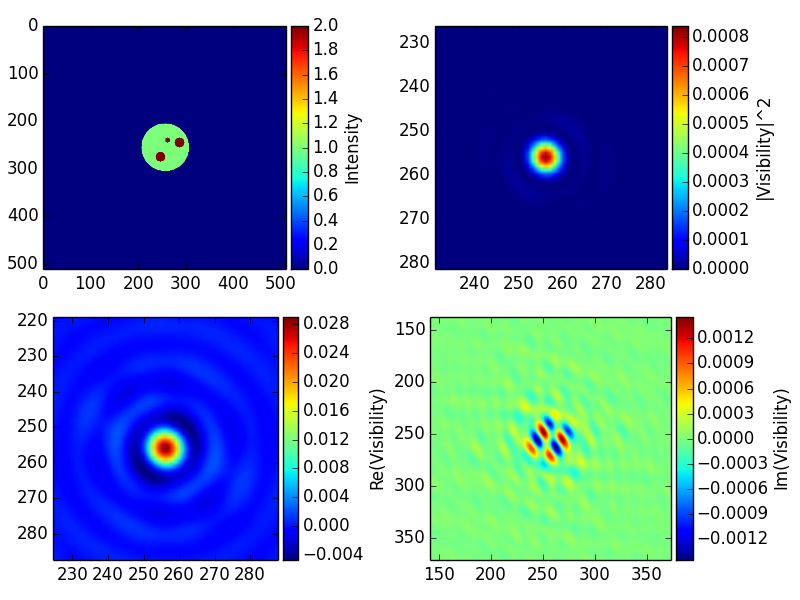
\includegraphics[scale=0.51]{figure_results_ptsized}
    \caption{Resulting signal at two detectors with radius 1 pixel (point-size detector approximation), slightly enlarged to see more details \label{fig:result_1px}
 }
\end{figure}

\begin{figure}[ht!]
	\centering
    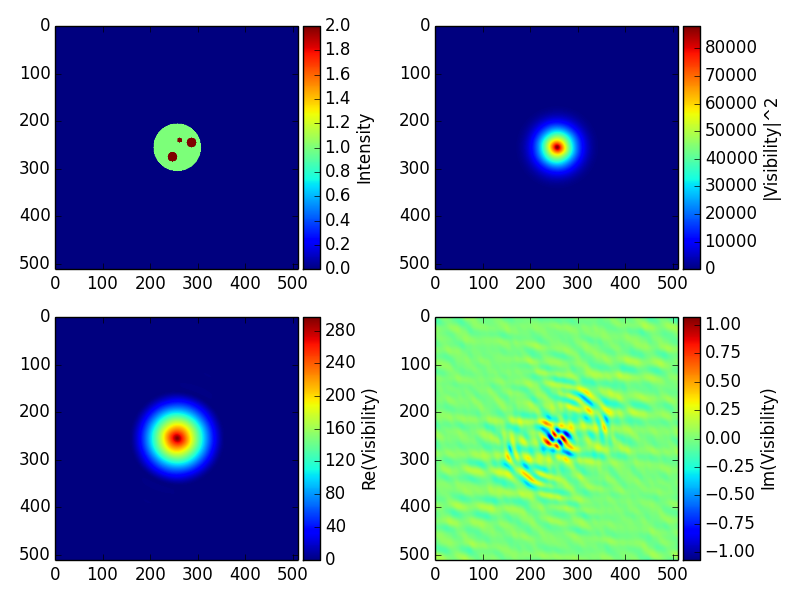
\includegraphics[scale=0.51]{figure_results}
    \caption{Resulting signal at two detectors, each with radius 50 pixels \label{fig:result_50px}
 }
\end{figure}
\section{Results}\label{results}

Plots of the source, the absolute squared visibility as well as the real and imaginary parts of the visibility can be seen in figure \ref{fig:result_50px} for detectors with a radius of 50 pixels and as a comparison in figure \ref{fig:result_1px} the same values for approximately point-sized detectors of radius 1 pixel. The grid size is 512*512 pixels.

%%%%%%%%%%%%%%%%%%%%%%%%%%%%%%%%%%%%%%%%%%%%%%%%%%%%%%%%%%%%%%%%%%%%%

\section{Interpretation and Conclusion}\label{conclusion}
In comparing the spatially-extended detector case to the point-size detector case, we find three big differences. Firstly, the measured absolute values get much bigger due to the bigger detector area. Secondly, the real part and the squared absolute visibility in particular get much bigger. Thirdly, in all three cases, the contrast gets worse. The first two effects are mostly due to the way the results were computed and would most likely be less important in a practical application due to the distances involved from source to detector and the relative size differences. The third effect however is interesting considering the substructure signal is still visible, albeit with a weaker contrast. This implies that it could indeed be possible to obtain useful results in practical applications. \\

\appendix
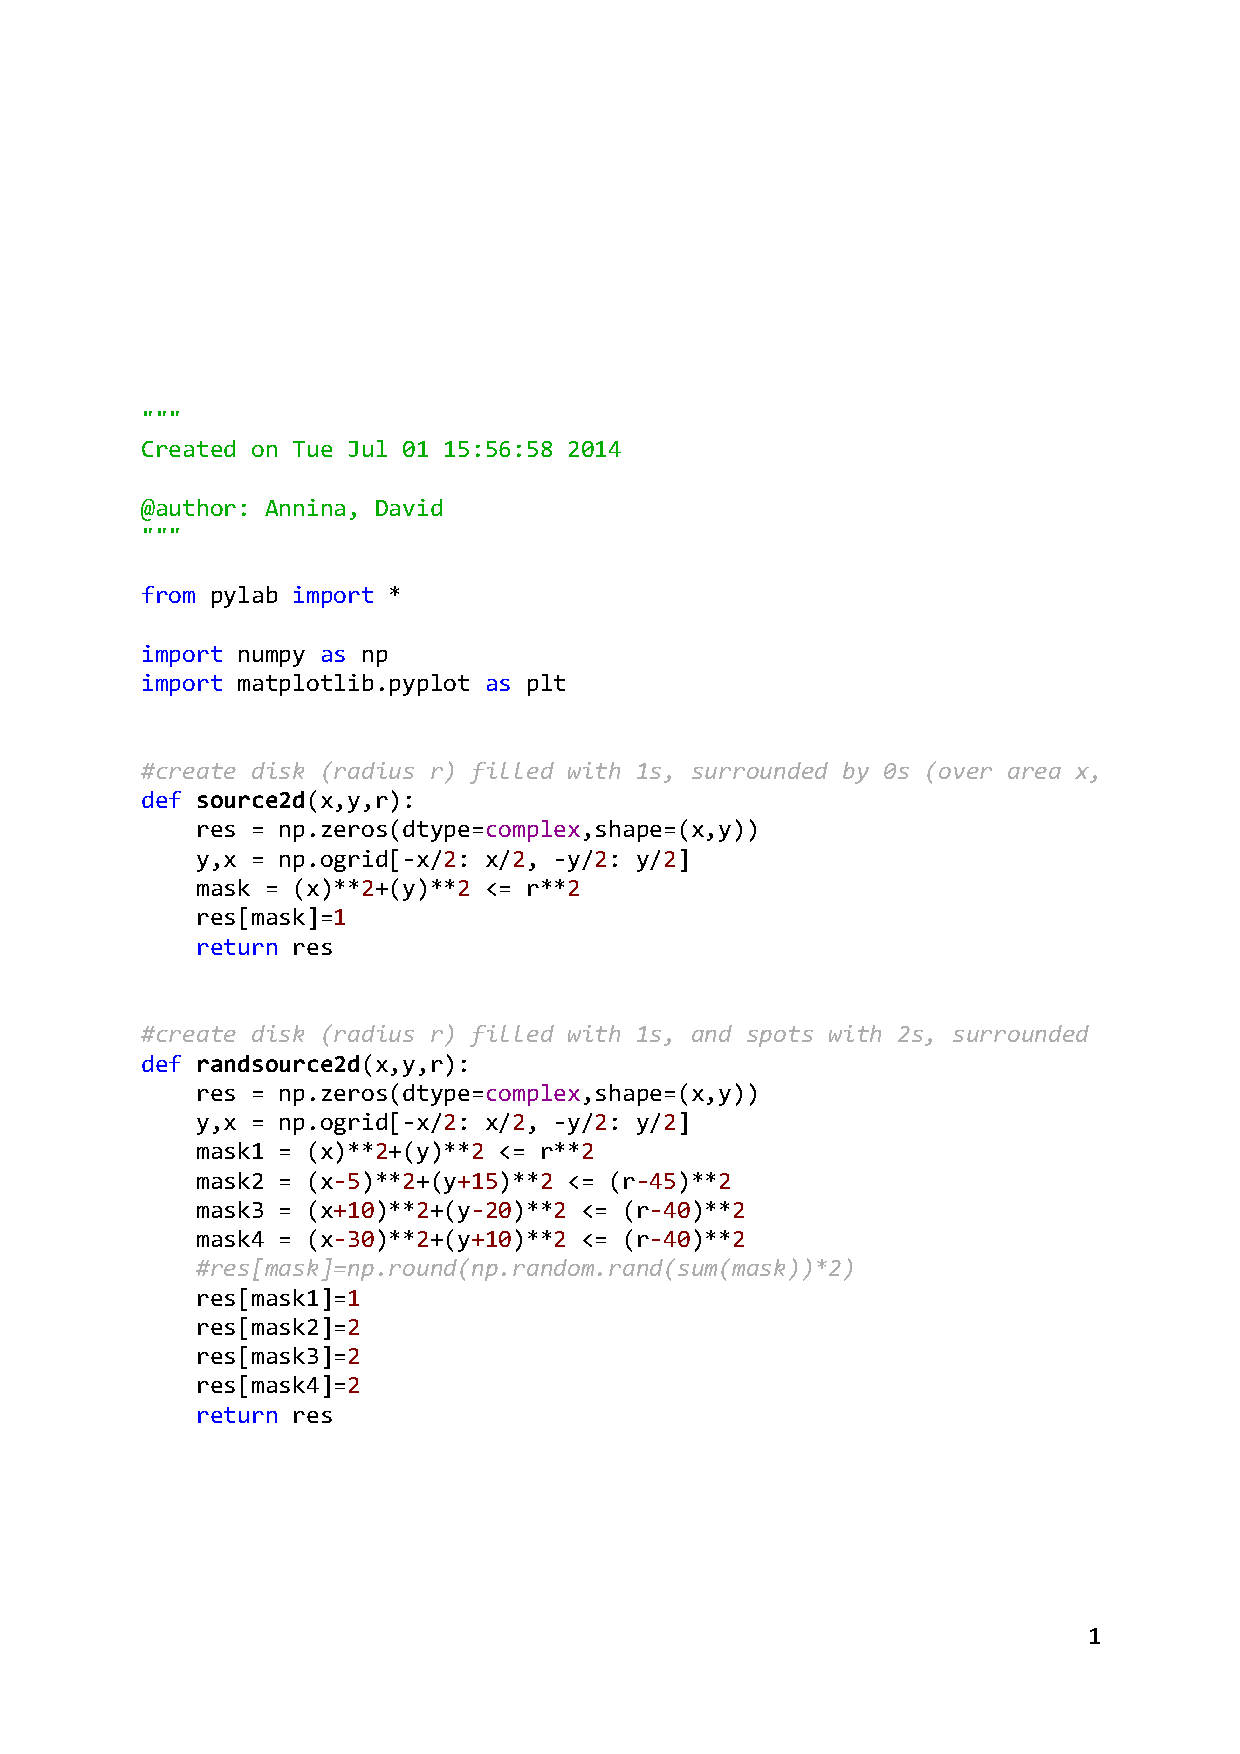
\includepdf[pages=1,pagecommand=\section{Python code used to obtain the results}]{appendix/code.pdf}\label{app:a}
\includepdf[pages=2,pagecommand={}]{appendix/code.pdf}

\bibliographystyle{plain}
\bibliography{report}

\end{document}
